\documentclass[a4,12pt]{scrartcl}
\usepackage{scrlayer-scrpage}
\usepackage[utf8]{inputenc}
\usepackage[english]{babel}
\usepackage{tcolorbox,url,xcolor}
\usepackage[bf,sf]{caption}
\DeclareCaptionLabelFormat{plain}{#2}
\captionsetup[figure]{labelformat=plain,labelsep=quad}

\begin{document}
\begin{flushright}
Felix Bühler, 1234567\\
Maximilian Wegge, 1234567\\
Carlotta Quensel, 3546286
\end{flushright}

\section*{Corpus Creation}
\subsubsection*{Emotion Analysis -- Assignment 1}
\subsection*{Data Selection}
For the task of annotating emotions, we considered different amazon review corpora and several reddit threads. The amazon reviews were discarded as they mostly contained sentiments rather than emotions. A possible solution of filtering out 'neutral' reviews with a medium number of stars would distort the observable emotions. Thus, the distribution in the corpus would not contain all possible emotions, which makes the corpus unsuitable for an exemplary emotion annotation. This also lead to the elimination of most reddit threads, as their domain often primed the users for a specific subset of emotions. We concluded to elect the reddit thread \textit{Redditors who live with their SOs, what changed?} for our annotation. The topic of this thread prompts users to describe emotional experiences and the question for \textit{change} also includes negative experiences. The data was scraped from \url{https://www.reddit.com/r/AskReddit/comments/5nrh7b/redditors_who_live_with_their_sos_what_changed/} and processed further using a python script. We removed deleted comments and users, subsequent conversations and bot answers, thus leaving the corpus with only comments directly answering to the question and containing around 500 documents. From those, the first 100 instances where used for the annotation task.

\subsection*{Annotation}
The annotation categories are modelled after Plutchik's wheel for its eight base categories and intensity rating were suitable for our specific data set. For the topic of \textit{change}, the emotions of surprise and anticipation were needed and the feature of forming 'cross-emotions' like love from neighboring categories opened up possibilities to further study the corpus. After annotation the first 10 instances, e chose to disregard Plutchik's intensity categories in favor of unnamed intensity scores. We also encountered the problem of latent emotions implied by the corpus domain, which is why we had to specify annotation rules for those specific categories. The resulting annotation guidelines contained the following information:

\begin{figure}
\centering
\begin{tcolorbox}
\textbf{\sffamily Annotation guidelines}

The annotation categories are Plutchik's eight base emotions of joy, sadness, trust, disgust, fear, anger, surprise and anticipation. The annotated value between 0 and 3 measures the intensity of the emotion label. The annotation environment has a document per line and eight columns for the emotion categories, thus every cell should contain a value. The categories are sorted as above with opposing emotions next to each other. Contrary to Plutchik's wheel is the annotation of opposing emotions in one document. This is possible due to the multi-label annotation and the perspective of the annotation.

As the data is related to the event of 'moving in together', most documents will likely contain event descriptions or event appraisals. Therefore, the annotator should assume the emotion felt in the described situation rather than at time of writing. This also includes comical exaggerations building to a punchline, which are annotated without regards to their intended readings. As the documents address living together with a romantic partner, joy and trust are likely to be implicit in many texts. Therefore, trust is in this context defined as an explicit referral to a positive relation to another person. This definition includes the negation, i.e. negative emotions due to the absence of another person but not statements that do not refer to a second person in any way.

\end{tcolorbox}
\caption{First iteration of the annotation guidelines}
\end{figure}

\begin{figure}
\centering
\begin{tabular}{l|cccccccc}
& joy & sadness & trust & disgust & fear & anger & surprise & anticipation\\\hline
anticipation & 1 & 0 & 1 & 0 & 0 & 1 &  0 & \textbf{2} \\
surprise  & 7 & 1 & 2 & 1 & 0 & 3 & \textbf{18} \\
anger & 1 & 2 & 1 & 1 & 0 & \textbf{18} \\
fear & 0 & 0 & 1 & 1 & \textbf{2} \\
disgust & 0 & 0 & 0 & \textbf{5} \\
trust & 6 & 1 & \textbf{16} \\
sadness & 1 & \textbf{5} \\
joy & \textbf{24}\\
\end{tabular}
\caption{Number of annotated documents using the average annotation and co-annotations of emotions}
\end{figure}

\begin{figure}
\centering
\begin{tabular}{l|cccc}
& \textbf{Felix} & \textbf{Carlotta} & \textbf{Max} & \textbf{\textit{average}}\\\hline
\textbf{joy} & 35 & 28 & 22 & \textit{28.33}\\
\textbf{sadness} & 11 & 6 & 4 & \textit{7.00}\\
\textbf{trust} & 21 & 23 & 16 & \textit{20.00}\\
\textbf{disgust} & 7 & 6 & 2 & \textit{5.00}\\
\textbf{fear} & 3 & 3 & 2 & \textit{2.67}\\
\textbf{anger} & 26 & 19 & 19 & \textit{21.33} \\
\textbf{surprise} & 43 & 24 & 19 & \textit{28.67} \\
\textbf{anticipation} & 10 & 15 & 3 & \textit{9.33} \\
\textbf{\textit{average}} & \textit{1.56} & \textit{1.24} & \textit{0.87} \\
\end{tabular}
\caption{Number of annotations per annotator and per category}
\end{figure}

% TODO: \usepackage{graphicx} required
\begin{figure}
	\centering
	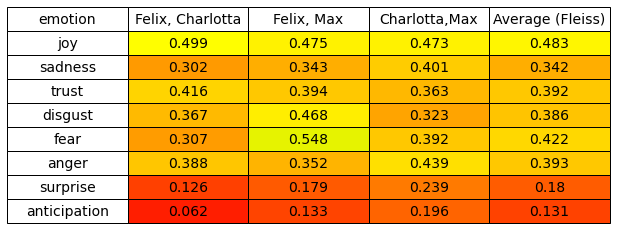
\includegraphics[width=0.7\linewidth]{emotion-eval-equal_distance}
	\caption[]{exact emotion}
	\label{fig:emotion-eval-equaldistance}
\end{figure}

\begin{figure}
	\centering
	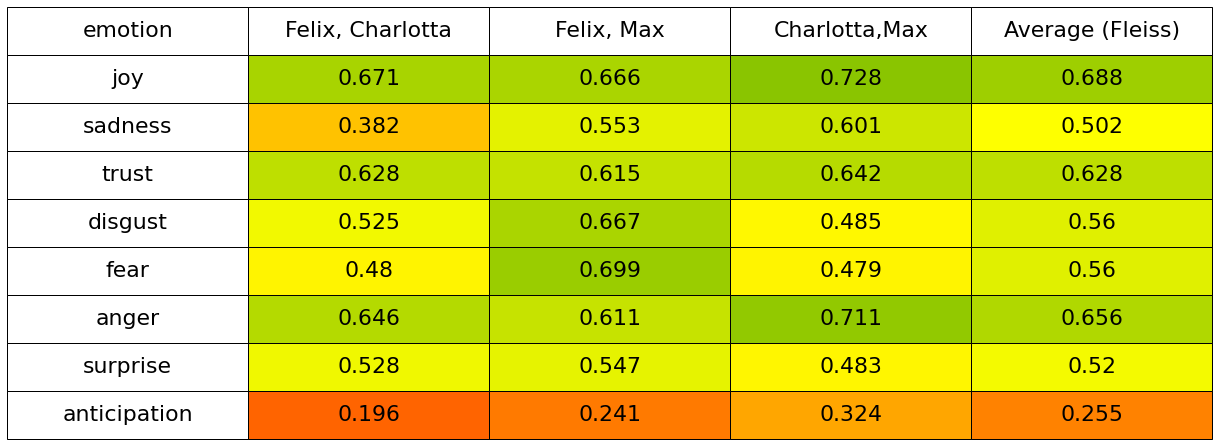
\includegraphics[width=0.7\linewidth]{emotion-eval-on_off_split}
	\caption[]{on/off-split emotion}
	\label{fig:emotion-eval-on_off_split}
\end{figure}

\begin{figure}
	\centering
	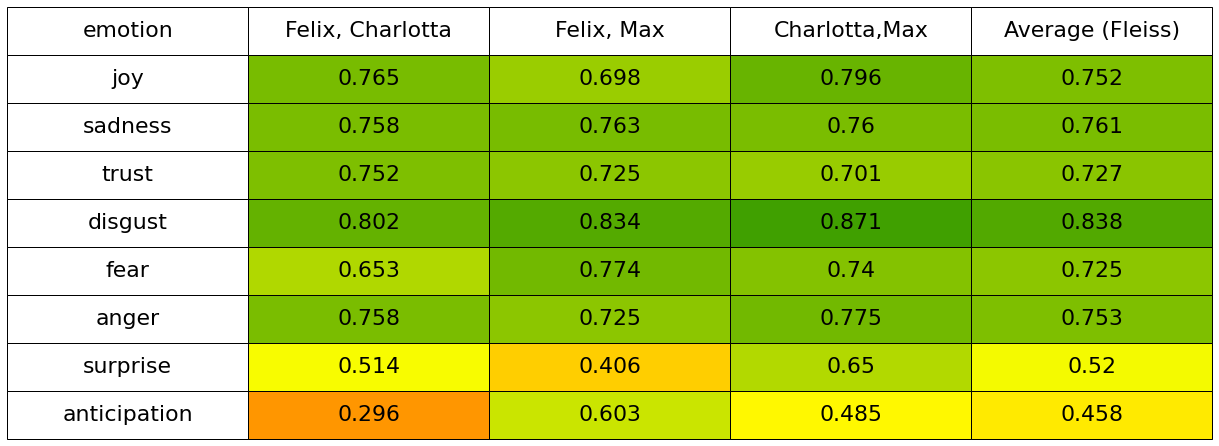
\includegraphics[width=0.7\linewidth]{emotion-eval-half_split}
	\caption[]{half-split emotion}
	\label{fig:emotion-eval-half_split}
\end{figure}



%%%%%%%%%%%%%%%%%%%%%Beispiele%%%%
\begin{center} % Beispiel mittig
\begin{tcolorbox}[width=40mm] %Breite manuell einstellen
\begin{itshape}
Example text is \colorbox{yellow}{here} % Farbliche Hinterlegung
\end{itshape}
\flushright \textbf{ID000} %docID am rechten Rand
\end{tcolorbox}
\end{center}
%%%%%%%%%%%%%%%%%%%%%%%%%%%%%%%%%%

\end{document}
